\newpage
\section{Water Quality Parameters} \label{variables}
In this section, multiple water quality parameters are described. A combination of these known parameters help with the evaluation of the total water quality in respect to different water applications such as surface water treatment and irrigation.

A small description of every parameter will be given, after which some sensors that may be suitable for mounting on the drone will be reviewed. Some multi parameter sensor systems will also be reviewed. In the following design report, a practical stack of some sensors will be made

%
%\subsection{Variables} 

%What are some useful things to know before surface water treatment?
%What is considered acceptable irrigation water?

%In the drone
\subsection{Temperature}
Temperature readings are used in the calculation of acidity, salinity, and in colorimetric tests. In limnological studies, knowledge of water temperatures as a function of depth often are required. The source of water supply, such as deep wells, often can be identified by temperature measurements alone. Surface water treatment plants also require data on water temperature at intake, as the viscosity of the water can differ. \cite{standardmethods}

\subsubsection{Sensors}
In this section, a comparison between potential temperature (℃) sensors for the project is given. Certain features like price, accuracy, and form factor will be given. The temperature sensors selected can be submerged in water.

\paragraph{DFRobot DFR0198/DS18B20}\mbox{€6,31} \cite{DFR0198}
\begin{table}[h!]
	\centering
	\adjustimage{height=4cm,valign=c}{water/41_dfr0198.jpg}\quad
	\begin{tabular}{| l | l |}
    \hline
    Protocol & 1-Wire\\
    Measurement Range & -10-85 ℃ \\
    Measurement Accuracy &  0.5 ℃ \\
    Response time & Within 750ms \\
    Supply Voltage & 3.3V-5V \\
    Software library included & yes \\
    Availability & 3-5 Working Days \\
    \hline
	\end{tabular}
\end{table}

\paragraph{Littelfuse USP10982}\mbox{€3,48} \cite{USP10982}
\begin{table}[h!]
	\centering
	\adjustimage{height=4cm,valign=c}{water/42_usp10982.jpg}\quad
	\begin{tabular}{| l | l |}
    \hline
    Protocol & Resistance (Analog)\\
    Measurement Range & 25-80 ℃ \\
    Measurement Accuracy &  0.55 ℃ after calibration\\
    Response time & Within 15s \\
    Software library included & no \\
    Availability & 3-5 Working Days \\
    \hline
	\end{tabular}
\end{table}
%In the drone
\newpage
\subsection{Acidity} \label{acidity}
Acidity is the quantitative capacity of a water or solution to neutralize an alkali. pH is a measure of the acidity or basicity of an aqueous solution. Solutions with a pH less than 7 are said to be acidic and solutions with a pH greater than 7 are basic or alkaline. \cite{phmerriam} Acidity can be interpreted in terms of specific substances only when the chemical composition of the sample is known. In this section, a closer look is taken at pH and how it affects the water quality. 

\subsubsection{Temperature}
The pH is inversely proportional to the temperature of the solution. When the temperature of a solution rises, the molecular vibrations in the solution rise resulting in the ionization and formation of H+ ions. More H+ ions lead to more acidic behavior. Generally, if we increase the temperature by 10°C, the pH of a solution or a substance will drop by 0.2.  \cite{temperatureph}

\subsubsection{Corrosion}
The pH is inversely proportional to the rate of corrosion. Corrosion occurs due to the formation of electrochemical cells. Low pH acid waters accelerate corrosion by providing a plentiful supply of hydrogen ions. The metal acts like an anode, with more negative potential with respect to the water which acts like a cathode. \cite{standardmethods}

\subsubsection{The carbon dioxide equilibrium system}
One of the most important chemical properties of water is that it can be both an acid and a base, because water ionizes into H+ and OH- ions.
The ionization is an equilibrium reaction.\\
The concentration of $H^+$ is usually denoted as the negative logarithm pH, while the concentration of $OH^-$ is denoted as the negative logarithm pOH.
For a neutral solution with a pH/pOH of 7.0 at 25 degrees celsius:
\[H^+ = OH^- = 0.0001 mmol/L\]
A lower pH than 7.0, meaning a higher concentration of H+ ions, indicates an acid solution. Water with a pH above 7 is a base. The pH of most raw water lies within the range 6.5–8.5 \cite{standardmethods}\\

The most important acid-base reaction in water is related to the dissociation of carbon dioxide. \cite{aes} When $CO_2$ becomes aqueous in water, a small portion of it becomes $H_2CO_3$, leaving $H^+$ ions:
\[CO_2 + H^2O <=> H^+ + HCO_3\]
$HCO_3^-$ can at it's turn release another $H^+$ ion:
\[HCO_3^- <=> CO_3^{2-} + H^+\]
The amount of carbon dioxide $CO_2$ in solution can determine the pH of the water. The most common source of acidity in water is dissolved $CO_2$, so the more $CO_2$ in the water, the lower the pH. As seen, dissolved $CO_2$ undergoes different stages over time. These stages have different pH levels associated with them:

\begin{figure}[h]
\centering
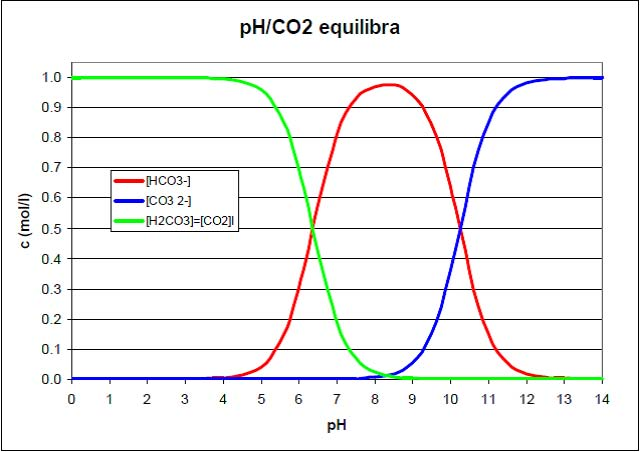
\includegraphics[scale=0.9]{water/21_equilibrium.jpg}
\caption{pH/$CO_2$ equilibrium \cite{aes}}
\end{figure}

\newpage
\subsubsection{Sensors}
In this section, a comparison between potential acidity (pH) sensors for the project is given. Certain features like price, accuracy, and form factor will be given.

To ensure accuracy, a pH probe needs to be calibrated first in two buffer solutions, pH 4.0 and pH 7.0. This has to be done every month. These buffer solutions usually cost around €15,- or can be found in most chemistry labs. As the pH is inversely proportional to the temperature of the solution, one should also use a temperature sensor to get meaningful data.

\paragraph{DFRobot Gravity V2}\mbox{€35.92} \cite{SEN0161V2}
\begin{table}[h!]
	\centering
	\adjustimage{height=4cm,valign=c}{water/22_gravityv2.jpg}\quad
	\begin{tabular}{| l | l |}
    \hline
    Interface & Analog \\
    Measurement Range & 0-14 pH \\
    Measurement Accuracy &  0.1pH \\
    Response time & Within 2min \\
    Supply Voltage & 3.3V-5V \\
    Software library included & yes \\
    Long term immersion & no \\
    Availability & 3-5 Working Days \\
    \hline
	\end{tabular}
\end{table}

\newpage
\paragraph{DFRobot Gravity V2 Pro}\mbox{€59,01} \cite{SEN0169V2}
\begin{table}[h!]
	\centering
	\adjustimage{height=4cm,valign=c}{water/23_gravityv2pro.jpg}\quad
	\begin{tabular}{| l | l |}
    \hline
    Interface & Analog \\
    Measurement Range & 0-14 pH \\
    Measurement Accuracy &  0.1pH \\
    Response time & Within 1min \\
    Supply Voltage & 3.3V-5V \\
    Software library included & yes \\
    Long term immersion & yes \\
    Availability & 3-5 Working Days \\
    \hline
	\end{tabular}
\end{table}


\paragraph{Generic PH0-14}\mbox{€15,83} \cite{PH0-14}
\begin{table}[h!]
	\centering
	\adjustimage{height=4cm,valign=c}{water/24_ph014.jpg}\quad
	\begin{tabular}{| l | l |}
    \hline
    Interface & Analog \\
    Measurement Range & 0-14 pH \\
    Measurement Accuracy &  0.25pH \\
    Response time & Within 1min \\
    Supply Voltage & 3.3V-5V \\
    Software library included & no \\
    Long term immersion & no \\
    Availability & 26 Days \\
    \hline
	\end{tabular}
\end{table}



\newpage
\subsection{Alkalinity}
Total alkalinity is a measurement of the water’s ability to resist a reduction in pH. Alkalinity ions resist reduction in pH by attracting a Hydrogen ion if needed. Total alkalinity is measured by the concentration (parts per million) in the water. \cite{standardmethods} In this section, a closer look is taken at total alkalinity and how it affects the water quality in different scenario's.

\subsubsection{Irrigation Water}
In order to evaluate the quality of irrigation water, one should know both pH and alkalinity. A pH test by itself is not an indication of alkalinity. Water with high alkalinity always has a pH value 7 or above, but water with high pH doesn't always have high alkalinity. 

Irrigating with water having a high pH causes no problems as long as the alkalinity is low (0 to 100 ppm calcium carbonate). The irrigation water will probably have little effect on growing medium pH because it has little ability to neutralize acidity.

Problems occur when water that has both high pH and high alkalinity is used for irrigation. The pH of the growing medium may increase significantly with time, decreasing crop rates. It is much more difficult to predict the effects of irrigating outdoor flower crops, gardens, and landscape plants with water having high pH and high alkalinity. 

Moderately alkaline water could be beneficial however as a source of extra $Ca$ and $Mg$ for crops prone to $Ca$ and $Mg$ deficiencies \cite{umassalkalinity}

\subsubsection{Water for aquatic life}
Fish and other aquatic life generally need a pH range of 6.5 to 8.0. \cite{fishphghkh} Since alkalinity buffers against rapid pH changes, the alkalinity helps protect the living organisms who need a specific pH range. Higher alkalinity levels in surface water can buffer acid rain and other acid wastes. This can prevent pH changes that are hazardous to aquatic life. 

%For drinking water?

\subsubsection{Sensors}

While there does exist a total alkalinity (ppm) sensor, it exists in the form of a lab-on-chip prototype developed by the national oceanography centre. \cite{alkalinitysensor} It is a bulky 6kg device meant to be used in large ships, and in no form suitable to be deployed in this project.

\paragraph{Lab-on-Chip Total Alkalinity Sensor}\mbox{} \cite{alkalinitysensor}
\begin{table}[h!]
	\centering
	\adjustimage{height=4cm,valign=c}{water/31_alkalinitysensor.jpg}\quad
	\begin{tabular}{| l | l |}
    \hline
    Measurement Range & 600umol/kg \\
    Measurement Accuracy &  5 umol/kg \\
    Response time & 12 min \\
    Supply Voltage & 10-16V \\
    Weight & 6kg \\
    Availability & Unknown \\
    \hline
	\end{tabular}
\end{table}

\newpage
%In the drone
\subsection{Conductivity}
Conductivity of a substance is defined as 'the ability or power to conduct or transmit heat, electricity, or sound'. \cite{merriamconductivity} Its units are Siemens per meter [S/m] in SI. Electrical conductivity is defined as the ratio between the current density (J) and the electric field intensity (e) and it is the reciprocal of the resistance:

\[s = J/e = 1/r\]

In water and ionic materials or fluids a net motion of charged ions can occur. This phenomenon produce an electric current and is called ionic conduction. Pure water is not a good conductor of electricity. Because the electrical current is transported by the ions in solution, the conductivity increases as the concentration of ions increases. \cite{lenntech} Conductance in water also depend on the mobility of the ions, the valence, and the temperature of the substance. \cite{standardmethods}\\


\subsubsection{Salinity}
In natural water, salinity is often determined by measuring the conductivity of the water. Typical values go as follows:

\begin{figure}[h]
\centering
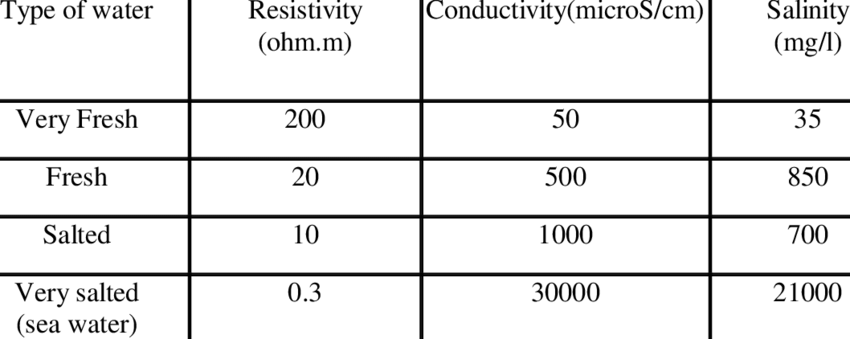
\includegraphics[scale=0.4]{water/61_typicalvalues.png}
\caption{Typical resistivity, conductivity and salinity values for different types of water \cite{abdulsamsudin}}
\end{figure}

\newpage
\subsubsection{Sensors}
In this section, a comparison between potential conductivity sensors for the project is given. Certain features like price, accuracy, and form factor will be given.

To ensure accuracy, a conductivity probe needs to be calibrated first in two buffer solutions of 1413us/cm and 12.88ms/cm. \cite{DFR0300H} This has to be done every month. These buffer solutions usually cost around €13,- or can be found in most chemistry labs.

\paragraph{Analog Devices EVAL-CN0349-PMDZ}\mbox{€49,04} \cite{CN0349}
\begin{table}[h!]
	\centering
	\adjustimage{height=4cm,valign=c}{water/62_cn0349.jpg}\quad
	\begin{tabular}{| l | l |}
    \hline
    Protocol & I2C\\
    Measurement Accuracy &  1\% FSR\\
    Supply Voltage & 3.3V\\
    Software library included & no \\
    Probe included & yes \\
    Availability & 2 Months \\
    \hline
	\end{tabular}
\end{table}

\paragraph{Gravity: Analog Electrical Conductivity Sensor}\mbox{€72,70} \cite{DFR0300H}
\begin{table}[h!]
	\centering
	\adjustimage{height=4cm,valign=c}{water/63_dfr0300h.jpg}\quad
	\begin{tabular}{| l | l |}
    \hline
    Protocol & Analog\\
    Measurement Accuracy &  5\% FSR\\
    Supply Voltage & 3.3-5V\\
    Support Detection Range & 10~100ms/cm\\
    Software library included & yes \\
    Probe included & yes \\
    Availability & 3-5 Working days \\
    \hline
	\end{tabular}
\end{table}
%In the drone
\newpage
\subsection{Turbidity}
Turbidity in water is caused by suspended and colloidal matter such as clay, silt, finely divided organic and inorganic matter, plankton and other microscopic organisms. Turbidity is an expression of the optical property that causes light to be scattered and absorbed rather than transmitted with no change in direction or flux level through the sample. \cite{standardmethods}\\

The unit measuring turbidity is known as NTU or JTU (Jackson Turbidity Unit):

\[1JTU = 1NTU = 1 mg/L\]


Clarity of water is important in producing products destined for human consumption and in many manufacturing operations. \cite{standardmethods} Water treatment plants drawing from a surface water source commonly rely on fluid-particle separation processes such as sedimentation and filtration to increase clarity and ensure an acceptable product.\\


\subsubsection{For aquatic life}

The clarity of a natural body of water is an important determinant of its productivity. Light penetration is especially important for submerged aquatic plants. These plants depend on light interception and absorption for photosynthesis. Enough light must be absorbed by the plant for photosynthesis to result in a net increase in biomass in order for the plant to grow and reproduce. 

Too much reductions in light levels result in death of the plant. As a result, plant growth in waters containing much turbidity and color is typically restricted to shallow depths, whereas plant growth is less restricted in less-turbid water. Submerged aquatic vegetation is a very important component of aquatic ecosystems. It provides food, shelter, and protection for many different aquatic species. Declines in this habitat will indirectly affect populations of species that depend on it. \cite{standardmethods}

\subsubsection{Using a multispectral camera}
As seen in \ref{similarprojects/multispectral} it is possible to get turbidity estimates by using a multispectral camera. This has the benefit of being able to cover a great amount of data in a short amount of time. It does require a lot of additional post processing to get realistic turbidity maps.

\subsubsection{Using a secchi disk}
A Secchi disk is a 30 cm disk with alternating black and white quadrants. It is lowered into the water until it can no longer be seen by the observer. This depth of disappearance, called the Secchi depth, is a measure of the transparency of the water. On an UAV, one could possibly use a RGB camera, a hoist, and machine vision to determine when the secchi depth is reached. \cite{secchidisk}

\newpage
\subsubsection{Sensors}
In this section, a comparison between potential turbidity sensors for the project is given. Certain features like price, accuracy, and form factor will be given.

As turbidity levels can change given depth, one should look into lowering these sensors at different depths.

\paragraph{DFRobot SEN0189}\mbox{€9.01} \cite{SEN0189}
\begin{table}[h!]
	\centering
	\adjustimage{height=4cm,valign=c}{water/71_sen0189.jpg}\quad
	\begin{tabular}{| l | l |}
    \hline
    Protocol & Analog\\
    Operating Temperature & 5-90 ℃ \\
    Operating Range &  0-3000NTU\\
    Response time & Within 500ms \\
    Supply Voltage & 0V-4.5V \\
    Software library included & yes \\
    Availability & 3-5 Days \\
    \hline
	\end{tabular}
\end{table}

\paragraph{Keyeyestudio KS0414}\mbox{€12.72} \cite{KS0414}
\begin{table}[h!]
	\centering
	\adjustimage{height=4cm,valign=c}{water/72_ks0414.png}\quad
	\begin{tabular}{| l | l |}
    \hline
    Protocol & Analog\\
    Operating Voltage & 5V\\
    Opearting Temperature & -30℃-80℃\\
    Operating Range & 0-4550NTU\\
    Measurement Accuracy & 228NTU\\
    Response time & Within 500ms \\
    Supply Voltage & 0V-4.5V \\
    Software library included & no \\
    Availability & 2 Weeks \\
    \hline
	\end{tabular}
\end{table}


\newpage
\subsection{Oxidation-Reduction Potential}
To reach a state of stability, substances that are lacking electrons are desperately seeking out electrons wherever they can. On the contrary, substances which have a surplus of electrons are capable of donating their extra electrons. These are called oxidizing and anti-oxidizing agents respectively.\\

Oxidation-reduction potential, or ORP, is a measurement that indicates the degree to which a substance is capable of oxidizing or reducing another substance. ORP is measured in millivolts.\cite{phorp} If the pH of water is higher than 9.5, then ORP meters become an invalid method of water quality measurement. \cite{standardmethods}

\subsubsection{Use in water treatment systems}
Water treatment is often accomplished through the addition of chlorine. The resulting oxidation reaction with water forms hypochlorous acid. In water treatment applications ORP is used to measure the oxidation by controlling the amount of free chlorine until a known bacteria killing ORP level is achieved. \cite{hamilton}

\subsubsection{Sensors}
In this section, a comparison between potential ORP sensors for the project is given. Certain features like price, accuracy, and form factor will be given.

\paragraph{DFRobot SEN0165}\mbox{€83,04} \cite{SEN0165}
\begin{table}[h!]
	\centering
	\adjustimage{height=4cm,valign=c}{water/81_sen0165.jpg}\quad
	\begin{tabular}{| l | l |}
    \hline
    Protocol & Analog\\
    Operating Temperature & 5-70 ℃ \\
    Operating Range &  -2000mV—2000mV\\
    Measurement Accuracy &  10mV \\
    Response time & Within 20s \\
    Supply Voltage & 5V \\
    Software library included & yes \\
    Availability & 3-5 Days \\
    \hline
	\end{tabular}
\end{table}

\paragraph{Generic ORP Sensor}\mbox{€50,58} \cite{orpsensor}
\begin{table}[h!]
	\centering
	\adjustimage{height=4cm,valign=c}{water/82_orpsensor.jpg}\quad
	\begin{tabular}{| l | l |}
    \hline
    Protocol & Analog\\
    Operating Temperature & 5-70 ℃ \\
    Operating Range &  -2000mV—2000mV\\
    Measurement Accuracy &  10mV \\
    Response time & Within 1min \\
    Supply Voltage & 5V \\
    Software library included & yes \\
    Availability & 26 Days \\
    \hline
	\end{tabular}
\end{table}
%Optionally in the drone
\newpage
\subsection{Total Dissolved Solids}
Total dissolved solids (TDS) can be defined as the mass of residue remaining when a measured volume of filtered water is evaporated. TDS is usually written in ppm (parts per million).

While turbidity is about particles that are not dissolved in water, total dissolved solids are about particles that are totally dissolved in water. TDS is usually low for freshwater sources, at less than 500 ppm. Seawater contains about 500-30,000 ppm, while brackish water contains 30–40,000 ppm.

\begin{figure}[h]
\centering
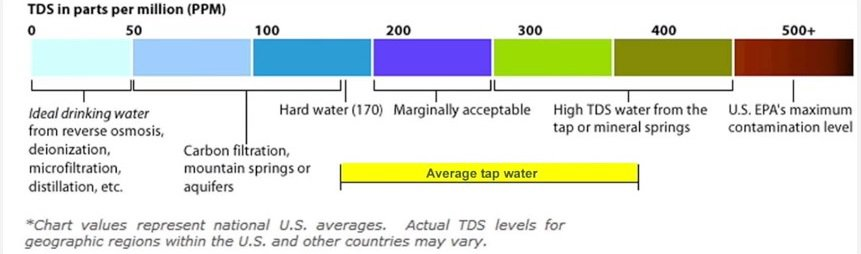
\includegraphics[scale=0.69]{water/91_tdschart.jpg}
\caption{TDS Chart for drinking water\cite{tdschart}}
\end{figure}

%Difference between conductivity sensor and tds sensor


\subsubsection{Sensors}
TDS sensors generally require temperature compensation in order to give accurate readings. Lower end models also generally require calibration from first use using a buffer solution of a known parts per million substance. \cite{sen0244wiki}

\paragraph{DFRobot SEN0244}\mbox{€11,66} \cite{SEN0244}
\begin{table}[h!]
	\centering
	\adjustimage{height=4cm,valign=c}{water/92_sen0244.jpg}\quad
	\begin{tabular}{| l | l |}
    \hline
    Protocol & Analog\\
    Operating Range & 0 ~ 1000ppm\\
    Measurement Accuracy &  100ppm \\
    Response time & Unknown \\
    Supply Voltage & 3.3V-5V \\
    Software library included & yes \\
    Availability & 3-5 Days \\
    \hline
	\end{tabular}
\end{table}

\newpage
\subsection{Multiparameter meter}
Multiparameter meters are instruments used to measure multiple electrochemical parameters at once. These may include methods for acidity, temperature, conductivity, turbidity, ORP, TDS, and more. All of the selected multiparameter meters are suitable for continuous testing in natural waters.

\paragraph{Aquaread AP2000}\mbox{} \cite{AP2000}
\begin{table}[h!]
	\centering
	\adjustimage{height=3cm,valign=c}{water/101_ap2000.jpg}\quad
	\begin{tabular}{| l | l | l |}
    \hline
    Variable & Range & Accuracy\\
    \hline
    DO & 0 – 50.00 mg/L & 0.01mg/L\\
    ORP & -2000 - 2000mV & 5mV\\
    Conductivity & 0 – 200mS/cm & 1\% FSR\\
    Acidity & 0 – 14pH & 0.01pH\\
    Temperature & -5C – +50C & 0.5C\\
    \hline
	\end{tabular}
\end{table}
\\The AP2000 can be fitted with additional optical or ion selective sensors to sense specific substances such as refined oil or ammonium. Values are saved on a standalone meter. One can retrieve sensor data from this meter and export it to CSV via a proprietary Windows application. It has a weight of 700g, excluding the meter.

\paragraph{PME Minidot}\mbox{} \cite{minidot}
\begin{table}[h!]
	\centering
	\adjustimage{height=3cm,valign=c}{water/102_minidot.jpg}\quad
	\begin{tabular}{| l | l | l |}
    \hline
    Variable & Range & Accuracy\\
    \hline
    DO & 0 – 50.00 mg/L & 0.3mg/L\\
    Temperature & 0C - 35C & 0.1C\\
    \hline
	\end{tabular}
\end{table}
\\One can retrieve real-time data from the logger via serial communication. The Minidot has a weight of 340g.

\paragraph{van Essen CTD Diver}\mbox{} \cite{ctddiver}
\begin{table}[h!]
	\centering
	\adjustimage{height=4cm,valign=c}{water/104_troll9500.png}\quad
	\begin{tabular}{| l | l | l |}
    \hline
    Variable & Range & Accuracy\\
    \hline
    Conductivity & 0 – 120 mS & 1\% FSR\\
    Temperature & 0C - 35C & 0.1C\\
    \hline
	\end{tabular}
\end{table}
\\After measurements, one can retrieve data from the logger via the included proprietary interface cable and Windows software. The CTD Diver has a weight of 95g.
\newpage
\paragraph{In-Situ TROLL 9500 Professional}\mbox{} \cite{AP2000}
\begin{table}[h!]
	\centering
	\adjustimage{height=3cm,valign=c}{water/101_ap2000.jpg}\quad
	\begin{tabular}{| l | l | l |}
    \hline
    Variable & Range & Accuracy\\
    \hline
    DO & 0-20-50 mg/L & 0.01-0.02-0.5mg/L\\
    ORP & -1400 - 1400mV & 5mV\\
    Conductivity & 0 – 200mS/cm & 0.5\% FSR\\
    Acidity & 0 – 12pH & 0.01pH\\
    Temperature & -5C – +50C & 0.5C\\
    \hline
	\end{tabular}
\end{table}
\\The TROLL 9500 is available in multiple editions with additional optical or ion selective sensors to sense specific substances such as ammonium, chloride, nitrate, and turbidity. Values are transmitted via the RS485/RS232 serial protocol. It has a weight of 1.9kg.